\chapter{Coding and layout construction}\label{ch:coding-and-layout-construction}

This chapter is the central part of the thesis
as it presents the novel genetic approach, which is demonstrated in solving the painting placement problem.
In section~\ref{sec:genetics}, definitions regarding genetics are laid out together with the Schema Theorem description.
Section~\ref{sec:coding} describing individual representation and section~\ref{sec:operators}
describing genetic operators together present the novel genetic approach.
Section~\ref{sec:reproductive-plan} describes the reproductive plan.
Lastly, section~\ref{sec:layout-construction} describes a greedy placing heuristic
used to construct the painting placement layout.

\section{Genetics}\label{sec:genetics}

This section describes critical genetic terms that are used throughout the thesis.
They are allele, gene, chromosome, individual, population, crossover, mutation, and reproductive plan.
Also, in subsection~\ref{subsec:schema-theorem}, the integral part of genetics called the Schema Theorem is described.

First, it is essential to describe what the genetic approach means.
The genetic approach was first introduced by Holland in 1975
to solve optimization problems where it is computationally infeasible to
find an optimal solution by enumerating all possible solutions~\cite{hollandAdaptationNaturalArtificial1975}.

This genetic approach is inspired by nature and Darwin’s Theory of Evolution
– a population of individuals evolving over time.
Individuals more adapted to the environment are
more likely to survive and thus pass their genes to the next generation.
Thus, over time, the population should converge to the state where the adaptation to the environment is the highest~\cite{darwinOriginSpeciesMeans2009}.

Holland in~\cite{hollandAdaptationNaturalArtificial1975} defines several structures that reassemble this natural process.
The most important ones are described in the rest of this section.\\

\navesti{Allele} represents a concrete value that a gene can have.
It can be thus described as a set of alternatives to choose from. \\

\navesti{Gene} is a structure composed of alleles.
It often describes one trait or characteristic. \\

\navesti{Chromosome} is a structure composed of genes.
Thus it is an amalgam of characteristics described by genes.\\

\navesti{Individual} is defined by its chromosome and represents a solution to the problem or a structure from which a solution can be constructed.
A numeric value called \definice{fitness} can be assigned to each individual, representing how well the individual performs in an environment. \\

\navesti{Population} is a set of individuals.
It can be interpreted as a subset of possible solutions.\\

One concrete example of the abovementioned definitions is in figure~\ref{fig:population}.
There are two individuals in the population, with their chromosomes having two genes.
The first gene is a vector containing permutation with alleles of 1 to 5.
The second gene is a string vector
with alleles having values $H$ or $V$.
Lastly, each individual has a fitness value.
Thus, because A’s fitness $30.5$ is greater than B’s fitness $9.8$, we can say that individual A performs better than B.


\begin{figure}
    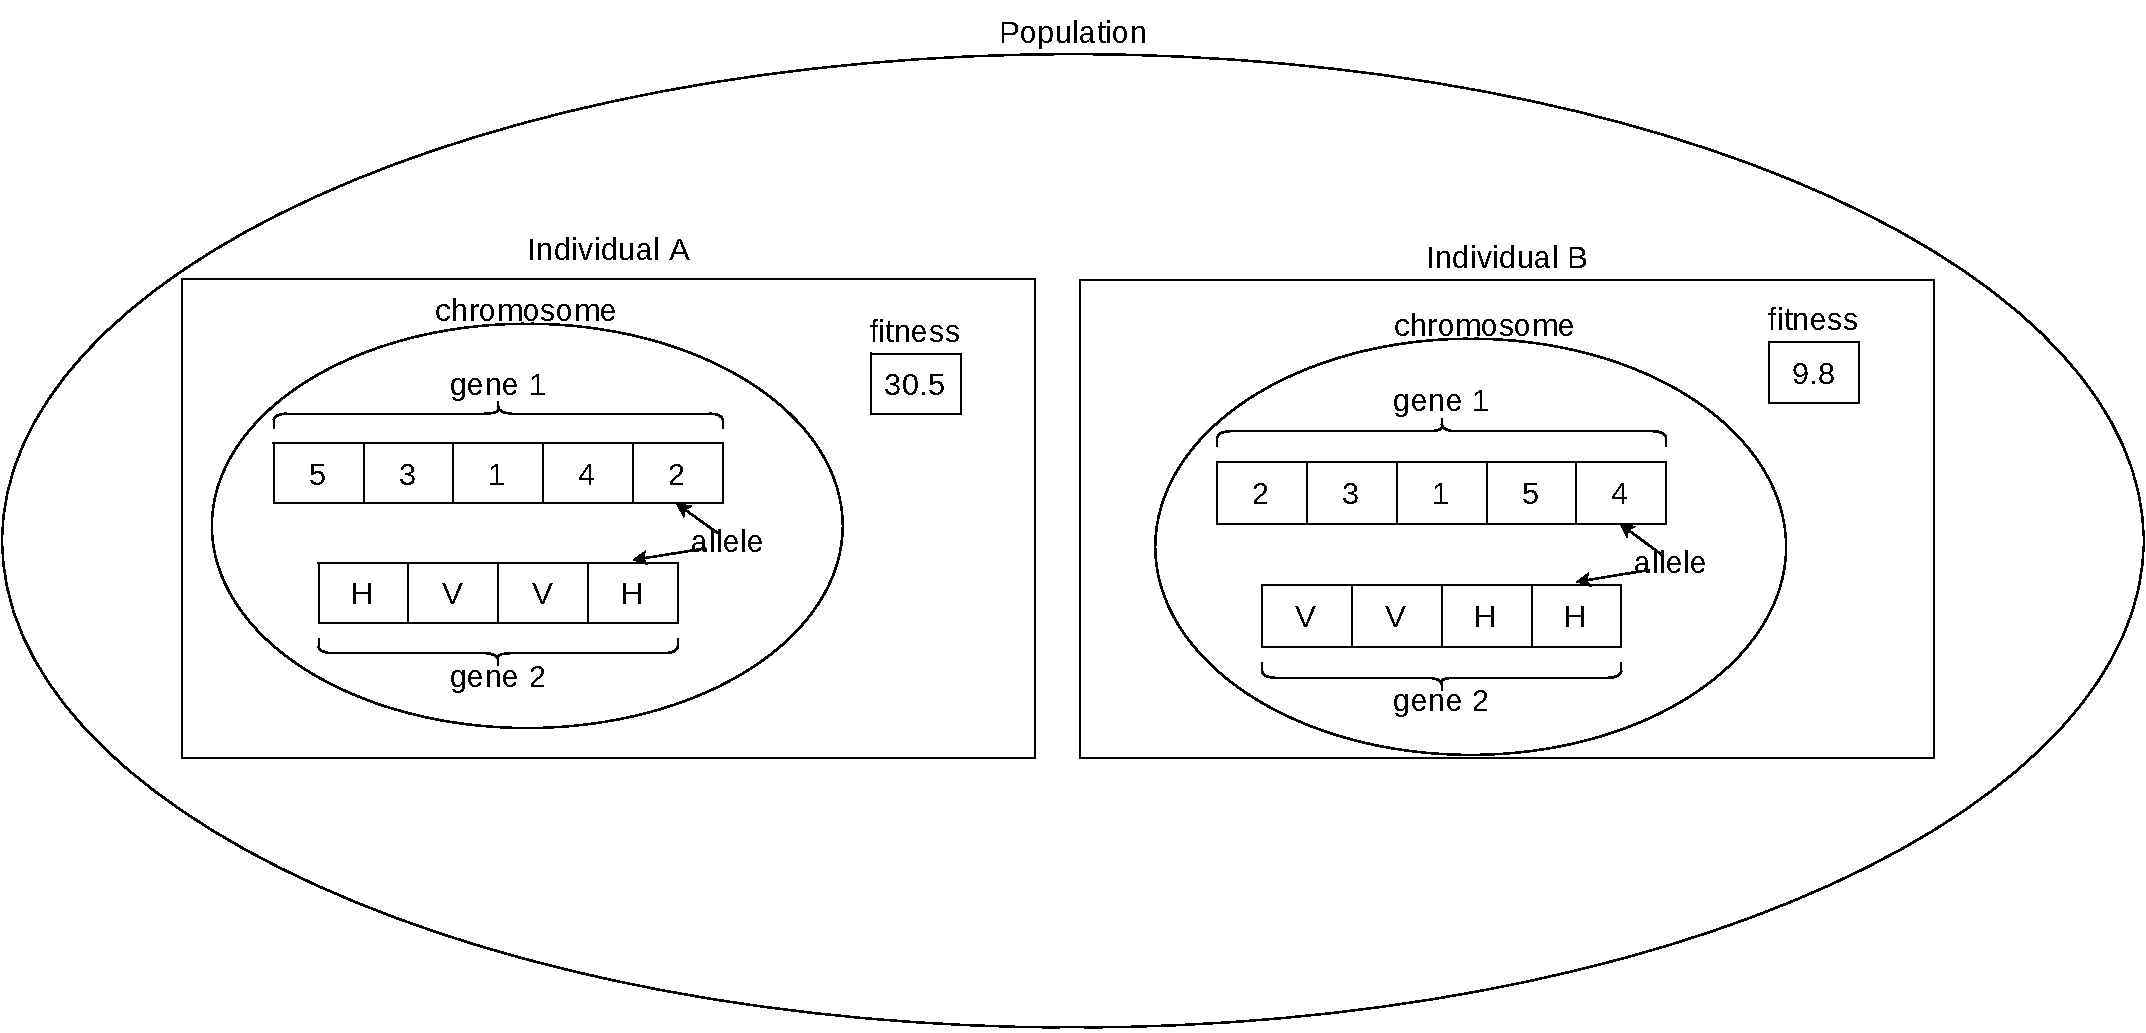
\includegraphics[width=1.1\textwidth, left]{population}
    \caption[Population example]{Example of a population composed of two individuals.}
    \label{fig:population}
\end{figure}

For the structures defined above, multiple operations called \definice{genetic operators} or simply operators
are defined by Holland and used by other researchers following his work.
Genetic operators aim to create new individual/s using individuals already present in a population as input.
Two of them that are used in this thesis are described below.\\


\navesti{Crossover} genetic operator takes two individuals as input and, by recombination
of their alleles in their genes, produces a new individual/s called \definice{offspring} or \definice{child}.\\

\navesti{Mutation} genetic operator takes one individual as input and produces a new one
which may have some of its alleles replaced by different ones at random.\\

Finally, there needs to be a process that transforms a population
to a new one with the goal of if this transformation process is applied sufficient
number of times to some initial population,
(sub)-optimal solution to the problem will be found.
This process is called the reproductive plan.\\

\navesti{Reproductive plan} is a process that takes a population on input and produces a modified
population using genetic operators.\\

One example of a reproductive plan is in figure~\ref{fig:reproductive-plan}.
At the start, an initial population of individuals is generated.
Then, for each individual, the fitness value is calculated.
Lastly, two genetic operators are applied to produce the new population.
In this example, crossover and mutation.
The process ends if the stopping condition is met.

\begin{figure}[h]
    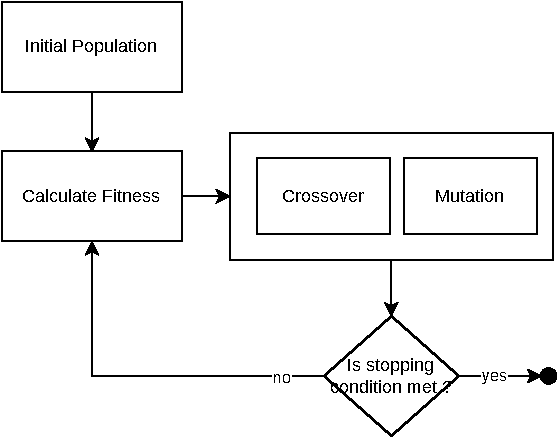
\includegraphics[width=0.65\textheight, center]{reproductive_plan}
    \caption[Example of a reproductive plan]{Example of a reproductive plan with crossover and mutation genetic operators.}
    \label{fig:reproductive-plan}
\end{figure}

\subsection{Schema Theorem}\label{subsec:schema-theorem}

Holland in~\cite{hollandAdaptationNaturalArtificial1975} proposed
the Schema Theorem arguing why the genetic approach described above works.
This subsection describes the main idea behind the argument.
First, an important term to describe is the schema.\\

\navesti{Schema} is an extended representation of chromosome,
where each gene can contain a “don’t care” symbol marked as underscore $\_$.
This symbol can take up any value that an allele can in the given context.
We can then say that chromosome belongs to a schema
and that schema contains a chromosome.\\

Schema can be illustrated on a chromosome with one gene represented as a vector that contains a permutation of numbers $1$ to $7$.
Then, example of a schema is $H_1 = \langle 5, \_, \_, 2, \_, 3, \_ \rangle$.
It contains $24$ chromosomes, with one example being $\langle 5, 4, 1, 2, 6, 3, 7 \rangle$.
On the other hand, schema $H_2 = \langle 1, 2, 3, 4, 5, 6, \_ \rangle$ contains only one chromosome.

There are two other properties that a schema has. They are length and order and are defined as follows.\\

\definice{Length} of a schema is the distance from the first “non-don’t care” symbol to the last.\\

\definice{Order} of a schema is the number of “non-don’t care” symbols contained in the schema.\\

For example, $H_1$ has length $6$ and order $3$.
It is graphically illustrated in figure~\ref{fig:schema}.
On the other hand, schema $H_2$ has the same length, $6$, but higher order, which is also $6$.

With schema being defined, we can interpret any population of individuals as a pool of schemata.
It can then be reformulated that a genetic approach, which has a reproductive plan and
genetic operators, (1) creates new schemata by recombination of the one already present in the population,
(2) creates schemata that are absent in the population, and (3) keeps a history of the best schemata found.
The Schema Theorem can then be written as

\begin{equation}
    \mathrm{E}[M(H, t+1)] \geq M(H, t) \dfrac{\mu(H)}{\overline{\mu}}\left[ 1 - p_c \dfrac{\delta(H)}{k-1} - \sigma(H)
    p_m \right]\,,
    \label{eq:schema-theorem}
\end{equation}

where $M(H, t)$ is expected number of individuals whose chromosome belongs to schema $H$ in population $t$,
$\mu(H)$ is average fitness of individuals whose chromosome belongs to $H$,
$\overline{\mu}$ is average population fitness,
$\delta(H)$ is length of schema $H$ with it’s maximum length $k$,
$\sigma(H)$ is order of $H$,
$p_c$ is crossover probability, and
$p_m \ll 1$ is mutation probability.

Inequality~\ref{eq:schema-theorem} says, that the success of a schema $H$,
considering only crossover and low probability mutation are purely determined
by its better-than-average performance, length, and order.
It can be thus said that the genetic approach favors
short schemata with low order that have better-than-average performance.

The reasoning behind the argument is that schemata with high order are more likely
to be damaged by mutation, i.e., an allele of a schema is replaced by a different one.
Also, longer schemata are more likely to be split using a crossover, whereas Holland
considers a one-point-crossover that produces an offspring’s chromosome by copying
of the first parent’s chromosome up to the crossover point, followed by the second parent chromosome after the crossover point.

\begin{figure}[h]
    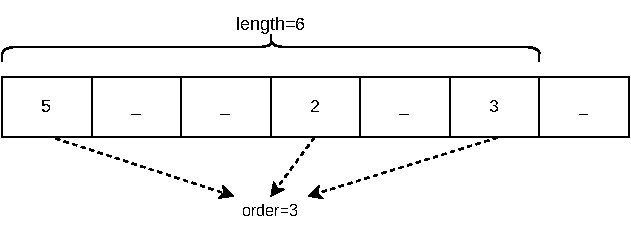
\includegraphics[width=0.7\textwidth, center]{schema}
    \caption[Example of a schema]{Example of a schema, where “don’t care” symbol marked as underscore $\_$.}
    \label{fig:schema}
\end{figure}

\section{Coding}\label{sec:coding}

The central part of the novel genetic approach proposed in this thesis is how an individual is represented.
This is important not only for the construction of the genetic operators, e.g., crossover and mutation
but also for the process of decoding an individual from its representation to the solution.

An individual is represented as a 3D chromosome—which means having three genes—that is composed of
(1) painting sequence random key, (2) slicing order random key, and (3) orientation probabilities.
An example of a chromosome is in figure~\ref{fig:chromosome}.

Let us use the notation for painting sequence random key as $PS_{rk}$,
slicing order random key as $SO_{rk}$,
orientation probabilities as $OR_{prob}$ and instance size as $N$, i.e., number of paintings.
First two are vectors, where $PS_{rk} \in \real^N$ and $SO_{rk} \in \real^{N-1}$.
Orientation probabilities is a matrix where $OR_{prob} \in \real^{N-1, 3}$.
Constraints in~\ref{eq:constraints} apply to each of these parts with
a stochastic vector meaning a vector that contains non-negative elements that add up to one.

\begin{equation}
    \begin{aligned}
        & 1. \quad PS_{rk} \text{ is a stochastic vector.} \\
        & 2. \quad SO_{rk} \text{ is a stochastic vector.} \\
        & 3. \quad \text{Each row in } OR_{prob} \text{ is a stochastic vector.}
    \end{aligned}\label{eq:constraints}
\end{equation}


The above-mentioned representation is based on a solution to the FLP
from~\cite{friedrichIntegratedSlicingTree2018, riponAdaptiveVariableNeighborhood2013},
where the authors represent an individual as a 3D chromosome with concrete identifiers for facilities, slicing order, and orientations.
However, the novel approach to coding proposed in this thesis are (1) the use of the stochastic vectors, (2) the use of random keys, (4) novel mutation and crossover operator, and
(3) introduction of novel decoding of an individual.
Thus, the search in the proposed genetic approach takes place in a different space, which is a space of stochastic vectors.

\begin{figure}[htp]
    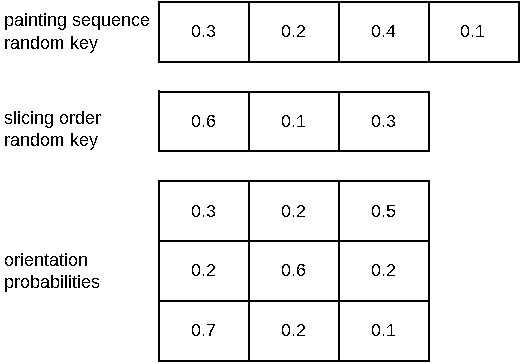
\includegraphics[width=0.8\textwidth, center]{chromosome}\caption[Example of an individual representation]{
        Example of an individual representation – two vectors and one matrix.
        Each vector and matrix row form a stochastic vector, i.e., they contain non-negative elements that add up to one.
    }
    \label{fig:chromosome}
\end{figure}

There are multiple ideas behind representing an individual as a set of stochastic vectors that stem
from extending RKGA~\cite{beanGeneticAlgorithmsRandom1994}, where chromosome is represented as a vector of values from $\langle0,1\rangle$.
First of them is the ability to perform mutation at an arbitrary element of these vectors using
a simple replacement, i.e., substituting an element for a random one from interval $\langle0,1 \rangle$,
followed by normalization back to the stochastic vector.
For example, using representation described in~\cite{friedrichIntegratedSlicingTree2018, riponAdaptiveVariableNeighborhood2013},
there has to be a different mutation method for each part of a chromosome.
By using the representation proposed in this thesis, there has to be only one mutation operator that can be used universally for all parts of the chromosome.

Additionally, when using representations similar to~\cite{friedrichIntegratedSlicingTree2018, riponAdaptiveVariableNeighborhood2013},
after the application of the genetic operators, usually crossover and mutation, an invalid individual might be created.
That is an individual that does not represent any solution.
The presence of invalid individuals might lead to performance loss in FLP~\cite{liuMultiimprovedGeneticAlgorithm2012}.
Moreover, unique solutions for dealing with invalid individuals must be introduced.
For example, left-to-right scan used by~\cite{hwangGeneticAlgorithmApproach2009, kandasamyEffectiveLocationMicro2020}
or leaving invalid individuals inside the population but penalizing them~\cite{hwangGeneticAlgorithmApproach2009}.
The solution proposed in this thesis produces only valid individuals.

Finally, the reasoning behind using a stochastic vector as opposed to a vector from $\langle0,1\rangle$ in RKGA~\cite{beanGeneticAlgorithmsRandom1994}
is the unique implementation of crossover used in this thesis, which is described in subsection~\ref{subsec:crossover}.

\section{Operators}\label{sec:operators}
As described in section~\ref{sec:genetics}, genetic operators are used to create
new individuals.
This section presents crossover and mutation genetic operators
that are used for the individual representation from section~\ref{sec:coding}.

\subsection{Crossover}\label{subsec:crossover}

Novel crossover approach proposed in this thesis
creates a new individual by weighted vector addition of the parent's stochastic vectors followed by a normalization back to the stochastic vector.
Using notation from section~\ref{sec:coding}, that is
$PS_{rk}$ for painting sequence random key vector,
$SO_{rk}$ for slicing order random key vector and
$OR_{prob}$ for orientation probabilities matrix,
we can define crossover for two parents $A$, $B$ and offspring $C$ as

\begin{equation}
    \|w_A A_{PS_{rk}} + w_B B_{PS_{rk}}\| = C_{PS_{rk}}\,,
    \label{eq:crossover-psrk}
\end{equation}

\begin{equation}
    \|w_A A_{SO_{rk}} + w_B B_{SO_{rk}}\| = C_{SO_{rk}}\,,
    \label{eq:crossover-sork}
\end{equation}

\begin{equation}
    \|P^T(w_A A_{OR_{prob}i:} + w_B B_{OR_{prob}i:})\| = C_{OR_{prob}i:}\,,
    \label{eq:crossover-orprob}
\end{equation}

where $\|\cdot\|$ is normalization to the stochastic vector, $+$ is vector addition, $w_A, w_B \in \real$ are weights,
$P \in \real^{N-1}$ is orientation penalization vector with $N$ being instance size, notation $X_{i:}$ means $i$-th row of a matrix $X$
and multiplying a vector by a scalar multiplies each element of the vector by that scalar.

Example of crossover for painting sequence random key and slicing order random key, eq.~\ref{eq:crossover-psrk} and~\ref{eq:crossover-sork},
is in figure~\ref{fig:crossover-random-keys}.
An example of crossover for orientation probabilities, eq.~\ref{eq:crossover-orprob}, is in figure~\ref{fig:crossover-orientation-probabilities}.

The crossover implementation described above has multiple parts – vector sum, weights, orientation penalization and normalization.
Following are arguments for incorporating each of those parts into a crossover.

\subsubsection*{Vector addition and normalization}

Adding and then normalizing vectors to stochastic vectors differs from other crossover implementations.
For example, in one-point-crossover~\cite{hollandAdaptationNaturalArtificial1975} and
uniform crossover~\cite{uniformCrossover1989}, parts of the parent chromosomes are copied directly without any modification to form an offspring.

\todo{poradny argument}


\subsubsection*{Weights}
Adding weights $w_A$ and $w_B$ determine the preference for transfer of information from one parent then the other.
The weights are calculated using a cost function $c$ from eq.~\ref{eq:objective} as

\begin{equation}
    w_A = \dfrac{c(B)}{c(A)+{c(B)}}, w_B = 1 - w_A\,.
    \label{eq:weights}
\end{equation}

Thus, parent with better performance in the population, i.e., having lower cost function,
has more influence on what genes are being transferred to the offspring.

Adding $w_A$ and $w_B$ prevents from creating offsprings that do not share the advantageous schemata.
For example, considering only one stochastic vector of length 3 as chromosome,
it might be advantageous having high value for the first value in the chromosome, e.g., $A=\langle 0.7, 0.1, 0.2 \rangle$.
On the other hand, poorly performing individual might be $B=\langle 0.1, 0.3, 0.6 \rangle$.
Without weights, $\| A+B\| = \langle 0.4, 0.2 , 0.4 \rangle$.
Adding weights according to the eq.~\ref{eq:weights} penalize the transfer of schemata that perform poorly.

\subsubsection*{Orientation penalization}

Another part of the crossover used in orientation probabilities matrix is the penalization vector $P$.
As mentioned in section~\ref{sec:layout-construction}, each individual is decoded to a slicing tree
whose internal nodes contain type of the cut – $H$ for horizontal, $V$ for vertical
and $*$ for wildcard, that can take up any value $H$ or $V$.
Vector $P$ controls the preference for each type of the cut.
For example, setting $P= \langle 1,1,0.5 \rangle$ penalize only the wildcard $*$.
On the other hand, setting $P= \langle 1,1,1 \rangle$ removes any penalization.

The main reason for introducing $P$ is to limit the spread of wildcard $*$ in population,
making its appearance only at the most advantageous parts of the genes.



\begin{figure}[htp]
    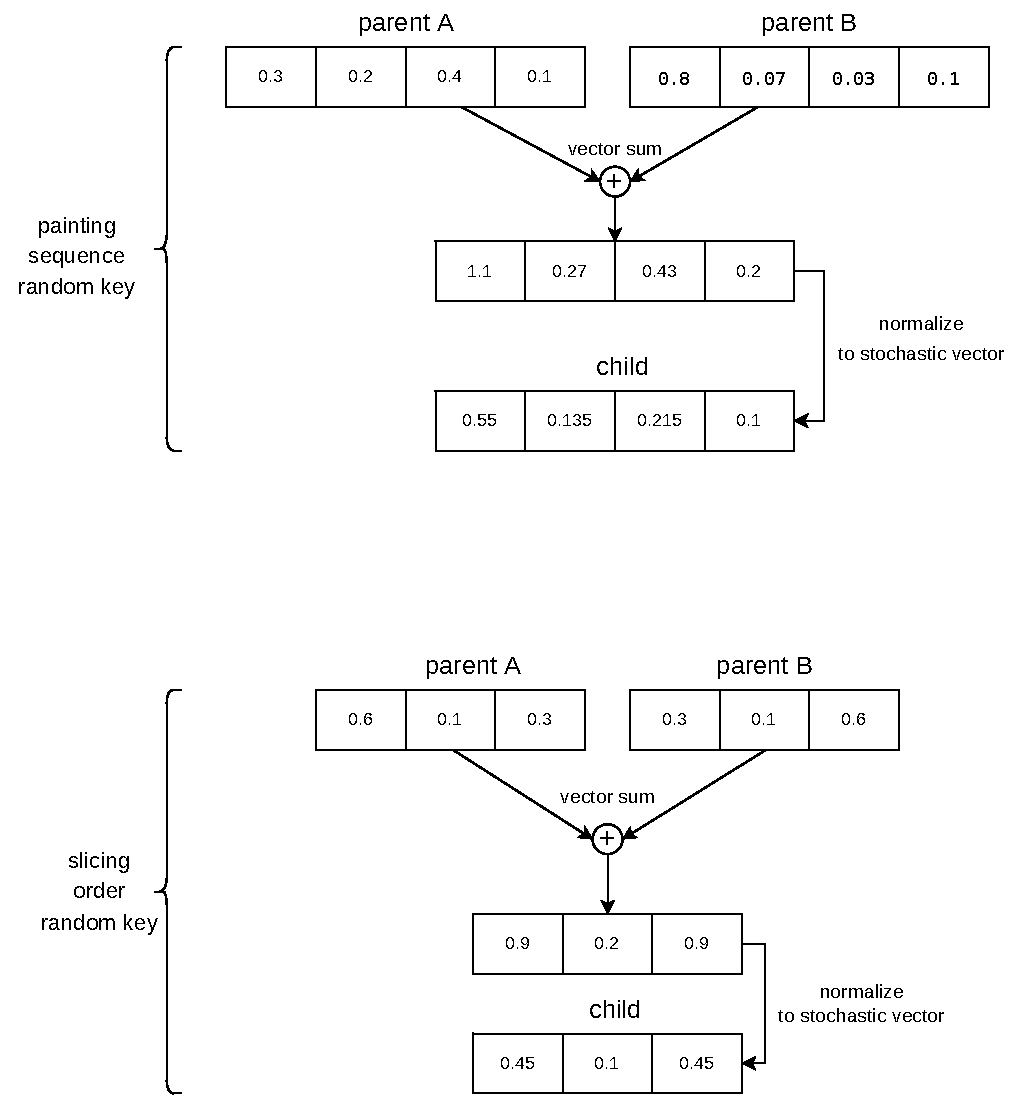
\includegraphics[width=1.0\textwidth, left]{crossover_random_keys}\caption{
        Crossover example for painting sequence and slicing order random keys.
        The procedure is the same for both – sum weighted parent vectors and then normalize to stochastic vector.
    }
    \label{fig:crossover-random-keys}
\end{figure}

\begin{figure}[htp]
    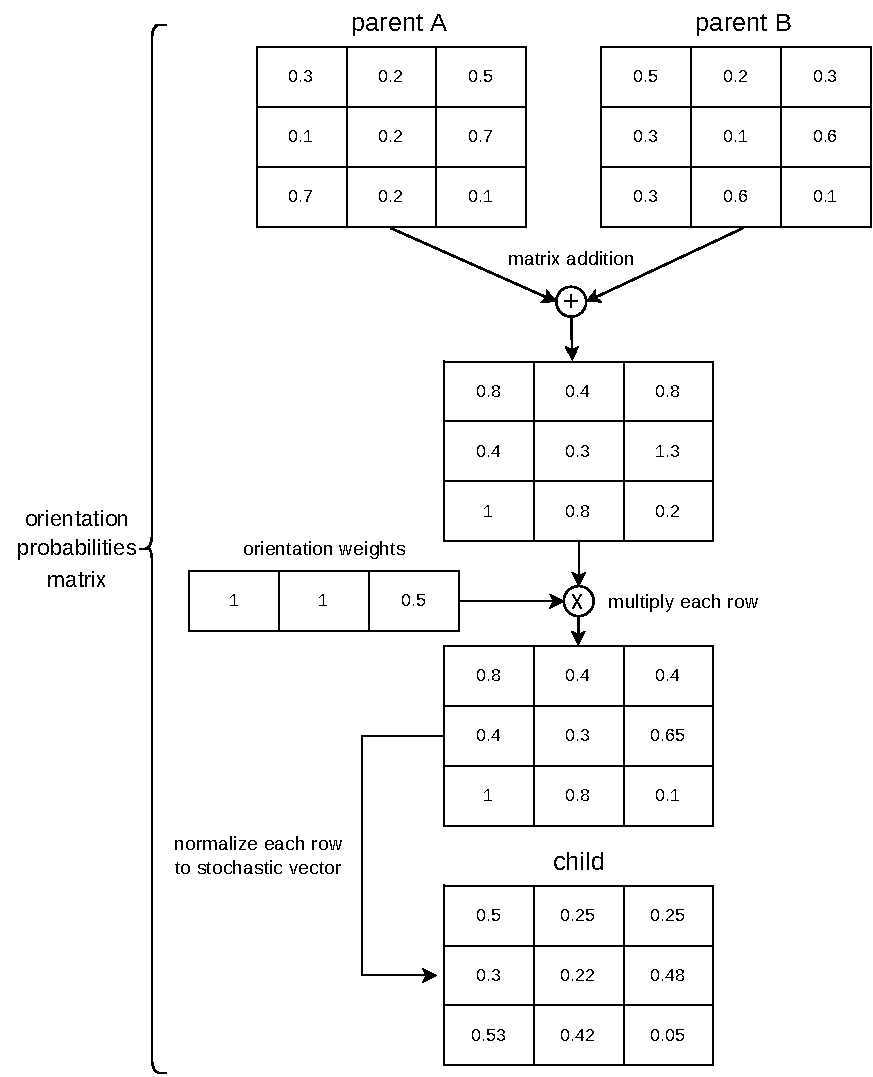
\includegraphics[width=0.85\textwidth, left]{crossover_orientation_probabilities}\caption{
        Crossover example for orientation probabilities. The procedure is first to sum weighted parent matrices,
        then multiply the matrix with orientation penalization vector and normalize each row to a stochastic vector.}
    \label{fig:crossover-orientation-probabilities}
\end{figure}

\subsection{Mutation}\label{subsec:mutation}

\section{Reproductive plan}\label{sec:reproductive-plan}
\section{Layout construction}\label{sec:layout-construction}

Solution to the painting placement problem is a set of placement points for the paintings.
There are multiple steps that transform the individual to these points.

\begin{enumerate}
    \item Decoding random keys and orientation probabilities.
    \item Slicing tree construction.
    \item Placement heuristic.
\end{enumerate}

In this section, the first two are described – decoding and slicing tree construction.
Last one, placement heuristic, is described in Chapter~\ref{TODO}.

\subsection{Individual decoding}\label{subsec:individual-decoding}
Goal of individual decoding is to transforms its representation to a different one,
which can be used to construct a slicing tree.

\subsection{Slicing tree construction}\label{subsec:slicing-tree-construction}

\subsection{Placement heuristics}\label{subsec:placement-heuristics}
